\documentclass[border=1mm]{standalone}
% \usepackage[margin=2.5cm]{geometry}

\usepackage{graphicx,tikz,tikz-layers,amsmath,ifthen,tabularray} 
\usetikzlibrary{decorations.markings,calc,positioning,arrows,shapes.geometric,arrows.meta,matrix}

\colorlet{myred}{red!80!black}
\colorlet{myblue}{blue!80!black}
\colorlet{mybluee}{myblue!80!black}
\colorlet{mygreen}{green!60!black}
\colorlet{myorange}{orange!70!red!60!black}
\colorlet{mydarkred}{red!20!black}
\colorlet{mydarkblue}{blue!40!black}
\colorlet{mydarkgreen}{green!20!black}




\begin{document}

% \resizebox{\textwidth}{!}{
\tikz[scale=1, every node/.style={outer sep=0pt, inner sep=0pt, align=center, rounded corners=0mm}, w/.style={minimum width=#1}, h/.style={minimum height=#1}, s/.style={minimum size=#1}, eu/.style={shorten >=#1}, ed/.style={shorten <=#1}, line join=round]
{
\tikzset{>={Latex[length=1.5mm, width=1.25mm]}}

\node[label={[label distance=1mm, font=\footnotesize]left:Original\\image}] (image) {\includegraphics[width=1.5cm]{images/parrot3-a.png}};

\node[draw, fill=myblue!15, w=2.45cm, h=5cm, right=.75cm of image, label={[label distance=2mm]above:$T$}] (t) {Data\\Augmentation};

\node[right=1cm of t.45, label={[label distance=1mm]above:$x_i$}] (image1) {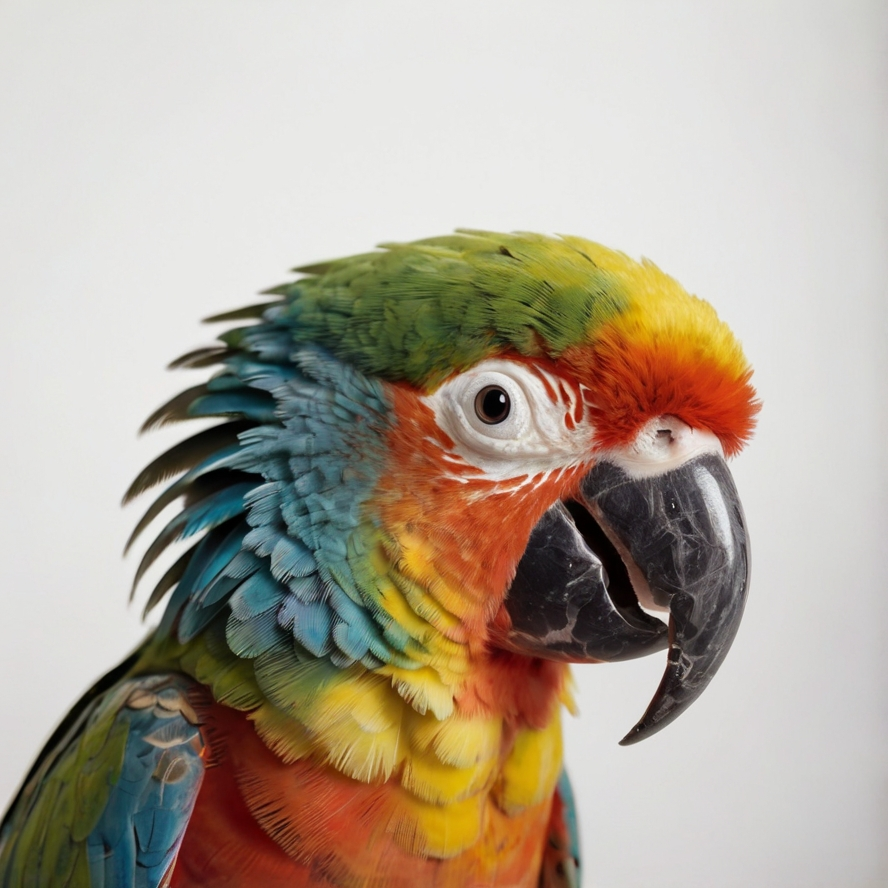
\includegraphics[width=1.5cm]{images/parrot5.jpg}};
\node[draw, right=1cm of image1, w=2cm, h=1cm, fill=mygreen!15] (enc1) {Encoder};
\node[draw, s=.5cm, fill=blue!50!cyan!15, right=1cm of enc1] (a1) {};
\node[draw, s=.5cm, fill=blue!50!cyan!15, right=0cm of a1, label={[label distance=2mm]above:$h_i$}] (a2) {};
\node[draw, s=.5cm, fill=blue!50!cyan!15, right=0cm of a2] (a3) {};
\node[draw, right=1cm of a3, w=1.5cm, h=1cm, fill=myblue!15] (den1) {Dense};
\node[draw, right=0cm of den1, w=1.5cm, h=1cm, fill=yellow!15] (rel) {Relu};
\node[draw, right=0cm of rel, w=1.5cm, h=1cm, fill=myblue!15] (den2) {Dense};
\node[draw, s=.5cm, fill=myred!15, right=.5cm of den2] (b1) {};
\node[draw, s=.5cm, fill=myred!15, right=0cm of b1, label={[label distance=2mm]above:$z_i$}] (b2) {};
\node[draw, s=.5cm, fill=myred!15, right=0cm of b2] (b3) {};
%-------------
\node[right=1cm of t.-45, label={[label distance=1mm]below:$x_j$}] (image2) {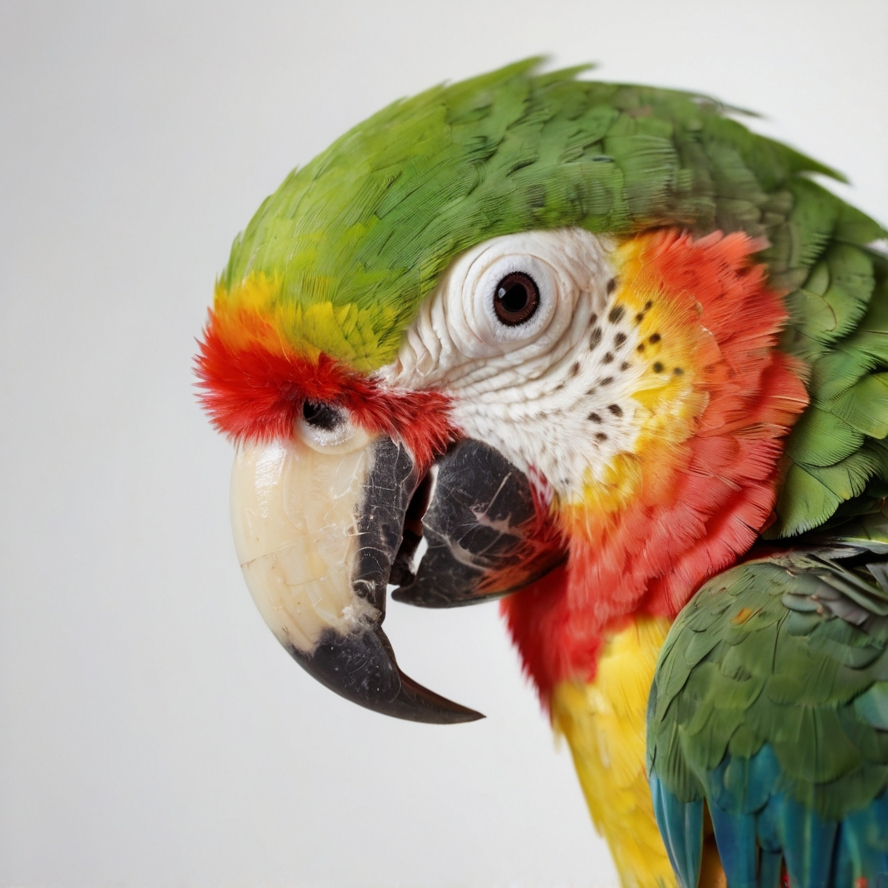
\includegraphics[width=1.5cm]{images/parrot4.jpg}};
\node[draw, right=1cm of image2, w=2cm, h=1cm, fill=mygreen!15] (enc2) {Encoder};
\node[draw, s=.5cm, fill=blue!50!cyan!15, right=1cm of enc2] (c1) {};
\node[draw, s=.5cm, fill=blue!50!cyan!15, right=0cm of c1, label={[label distance=2mm]below:$h_j$}] (c2) {};
\node[draw, s=.5cm, fill=blue!50!cyan!15, right=0cm of c2] (c3) {};
\node[draw, right=1cm of c3, w=1.5cm, h=1cm, fill=myblue!15] (den3) {Dense};
\node[draw, right=0cm of den3, w=1.5cm, h=1cm, fill=yellow!15] (rel1) {Relu};
\node[draw, right=0cm of rel1, w=1.5cm, h=1cm, fill=myblue!15] (den4) {Dense};
\node[draw, s=.5cm, fill=myred!15, right=.5cm of den4] (d1) {};
\node[draw, s=.5cm, fill=myred!15, right=0cm of d1, label={[label distance=2mm]below:$z_j$}] (d2) {};
\node[draw, s=.5cm, fill=myred!15, right=0cm of d2] (d3) {};

\node[draw, fill=myblue!15, w=2.45cm, h=1cm, below=1.5cm of c2] (dt) {Downstream\\tasks};
% Gray background boxes
\begin{scope}[on behind layer]
\node[draw, fill=gray!10, w=2.45cm, h=5cm, label={[label distance=1mm, font=\footnotesize]above:Transformed\\image}, anchor=north] at (t.north-|image1){};    
\node[draw, fill=gray!10, w=2.45cm, h=5cm, label={[label distance=1mm, font=\footnotesize]above:Base Encoder\\$f(.)$}, anchor=north] at (t.north-|enc1){};
\node[draw, fill=gray!10, w=2.45cm, h=5cm, label={[label distance=2mm, font=\footnotesize]above:Representation}, anchor=north] (u) at (t.north-|a2){};
\node[draw, fill=gray!10, w=4.95cm, h=5cm, label={[label distance=1mm, font=\footnotesize]above:Projection Head\\$g(.)$}, anchor=north] at (t.north-|rel1){};
\end{scope}

% Arrows
\draw[->] (image.north) |- (t.180-50);
\draw[->] (image.south) |- (t.180+50);
\draw[] (image1.west)--(image1.west-|t.east);
\draw[->] (image1)--(enc1)--(a1) (a3)--(den1) (den2)--(b1);
\draw[] (image2.west)--(image2.west-|t.east);
\draw[->] (image2)--(enc2)--(c1) (c3)--(den3) (den4)--(d1);
\draw[rounded corners=1mm] (b3.east)--++(.5,0) |- node[pos=.25,left=1mm, font=\footnotesize] {Maximize\\similarity} (d3);
\draw[->] (u)--(dt);

}

% }



\end{document}
